\newpage
\section{Valutazione dei dataset}
Durante la ricerca per trovare dataset gratuiti utilizzabili per l'addestramento del modello,
oltre a quelli messi a disposizione dall'azienda, si è trovato il dataset 
\cite{guillem_montalban_faet_2025_17866344}. Tuttavia, questo non contiene il canale SWIR e inoltre le immagini contenute sono state scattate da un drone e non da un satellite.
Si cercava infatti dei dataset differenti da quelli forniti dall'azienda per diversificare le fonti e di conseguenza migliorare la conoscenza del modello.

Per valutare la bontà dei dati e per comprendere se un ipotetico classificatore è in grado di distinguere i vari pixel si sono costruiti i grafici rappresentanti i valori delle bande.
Si mostrano di seguito i plot.
Nello specifico si sono create delle bbox di diverse tipologie:
\begin{itemize}
    \item bbox per indicare le non piante (sfondo)
    \item bbox per indicare le piante avocado
    \item bbox per indicare le piante di un'altra tipologia (1)
    \item bbox per indicare le piante di un'altra tipologia (2)
\end{itemize}
Le bbox (Bounding Box) sono riquadri di ritaglio nell'immagine su cui si è lavorato.
Le bbox che etichettano la pianta avocado sono state create utilizzando una fotografia RGB scattata 
da un drone quando la pianta era piccola. Questa immagine è stata data in input 
a un modello aziendale che lavora con l'RGB ad alte risoluzioni. 
Questo modello identificava tutte le piante presenti e solo in un secondo momento si è effettuata un pulizia manuale delle piante che non erano pertinenti.
A questo punto le bbox sono state inserite nell'immagine satellitare.
Il dataset \cite{guillem_montalban_faet_2025_17866344} invece è già stato spezzettato e quindi non sono state apportate modifiche da quel punto di vista.
Tutta le altre bbox (sfondo, tipologia2 e tipologia3) sono state disegnate a mano.
Si rivelano delle foto che manifestano la complessità e il lungo lavoro svolto in questa fase \ref{fig:satellitaresenzabbox} \ref{fig:satellitareconbbox}.
\begin{figure}[H]
    \centering
    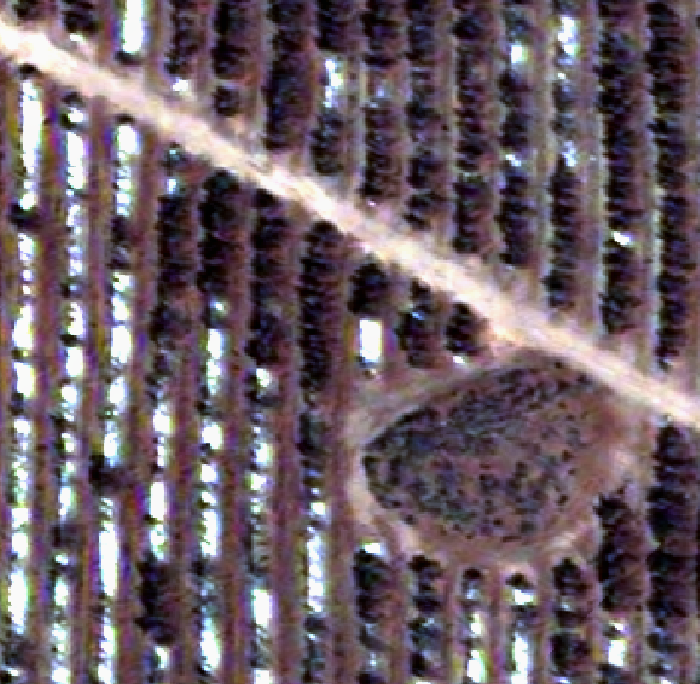
\includegraphics[width=0.55\textwidth]{capitoli/capitolo2/images/bbox/satellitare_senzabbox.png}
    \caption{Si mostra un immagine satellitare di un campo. Si noti la scarsa visibilità e la fatica a individuare la pianta}
    \label{fig:satellitaresenzabbox}
\end{figure}
\begin{figure}[H]
    \centering
    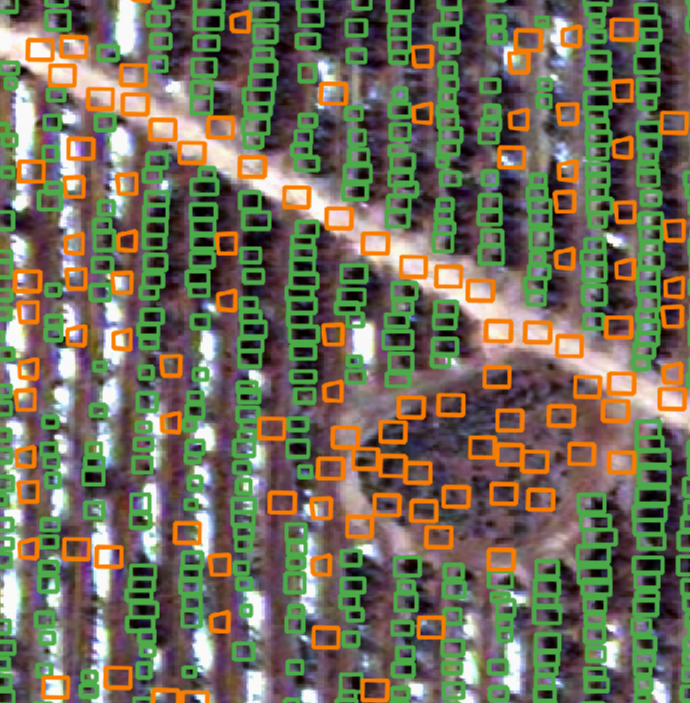
\includegraphics[width=0.55\textwidth]{capitoli/capitolo2/images/bbox/satellitare_conbbox.png}
    \caption{Si mostra l'immagine precedente \ref{fig:satellitaresenzabbox} con le bbox disegnate. Le bbox di colore verde sono le piante di avocado identificate dal modello RGB. In arancione sono raffigurate le bbox (disegnate a mano) che etichettano lo sfondo}
    \label{fig:satellitareconbbox}
\end{figure}
Per ogni bbox di una tipologia si genera il grafico dei pixel contenuti all'interno della bbox.\\
Di seguito si mostrano i plot per quanto riguarda le bbox non piante e le bbox
che contengono le piante avocado \ref{fig:plotavocadoRGB}

%inizio dei plot
\begin{figure}[htbp]
    \centering
    \begin{minipage}{0.30\textwidth}
    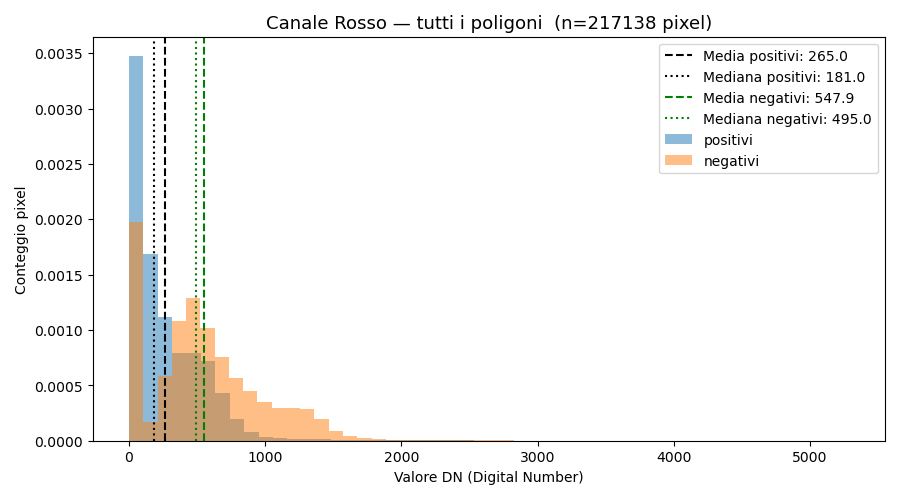
\includegraphics[width=0.9\textwidth]{capitoli/capitolo2/images/avocado/Satelliterosso.png}
    \end{minipage}
    \hfil 
    \begin{minipage}{0.30\textwidth}
    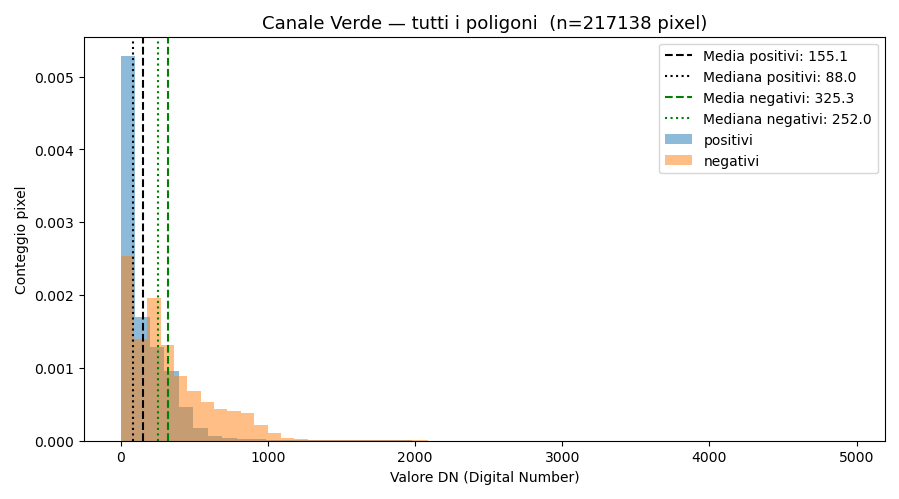
\includegraphics[width=0.9\textwidth]{capitoli/capitolo2/images/avocado/Satelliteverde.png}
    \end{minipage}
    \hfil
    \begin{minipage}{0.30\textwidth}
    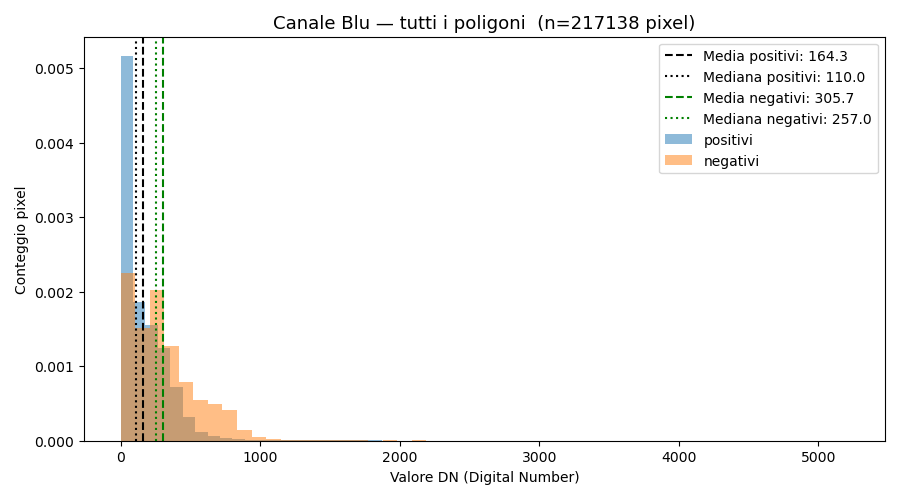
\includegraphics[width=0.9\textwidth]{capitoli/capitolo2/images/avocado/Satelliteblu.png}
    \end{minipage}
    \caption{Si mostrano i grafici RGB delle bbox degli avocado e dei non pianta}
    \label{fig:plotavocadoRGB}
\end{figure}

Di seguito si mostrano i plot delle bande dell'infrarosso (RedEdge, NIR, SWIR) \ref{fig:plotavocadoInfrarosso}:
\begin{figure}[htbp]
    \centering
    \begin{minipage}{0.30\textwidth}
    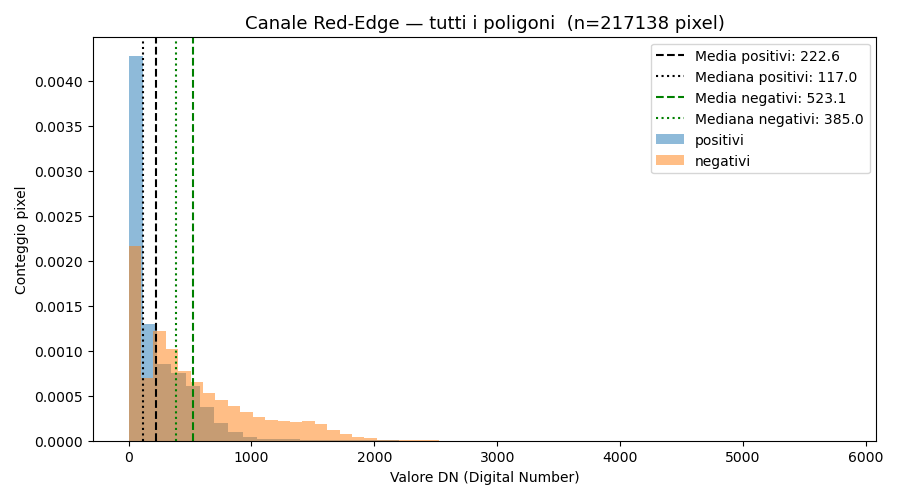
\includegraphics[width=0.9\textwidth]{capitoli/capitolo2/images/avocado/SatelliteRedEdge.png}
    \end{minipage}
    \hfil 
    \begin{minipage}{0.30\textwidth}
    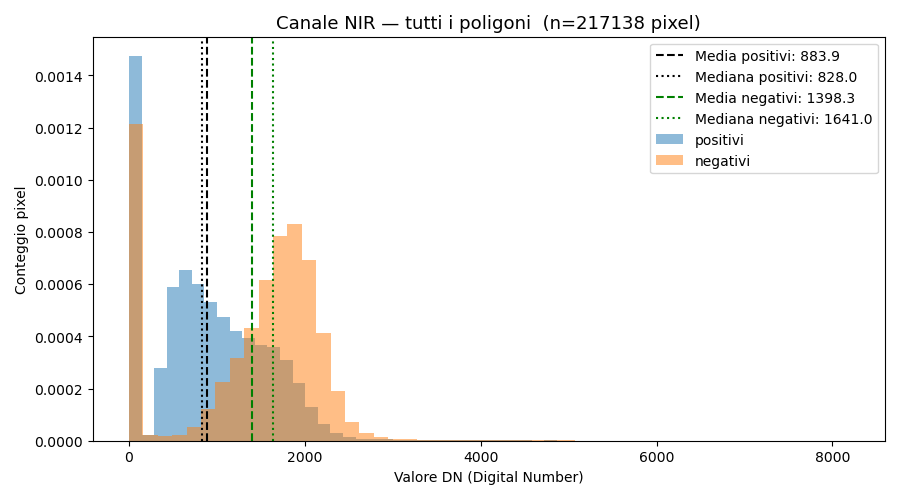
\includegraphics[width=0.9\textwidth]{capitoli/capitolo2/images/avocado/SatelliteNIR.png}
    \end{minipage}
    \hfil
    \begin{minipage}{0.30\textwidth}
    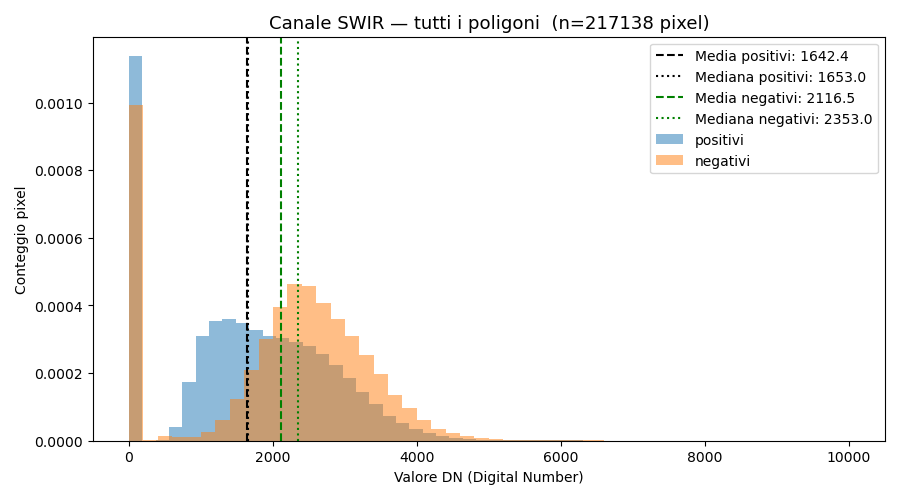
\includegraphics[width=0.9\textwidth]{capitoli/capitolo2/images/avocado/SatelliteSWIR.png}
    \end{minipage}
    \caption{Si mostrano i grafici infrarosso delle bbox degli avocado e dei non pianta}
    \label{fig:plotavocadoInfrarosso}
\end{figure}

Dato che i valori (prossimi allo 0) rendono il grafico poco chiaro e per via di istogrammi combacianti a interpretare le differenze, 
si è deciso di
rimuoverne alcuni di questi valori per rendere il grafico interpretabile.

Come si evince dai grafici in quasi tutte le bande gli istogrammi sono quasi tutti sovrapposti. 
Si riesce a differenziare solo nelle 2 classi (avocado e non pianta) solo nelle bande dei grafici NIR e SWIR.
Questa separazione, sebbene non netta, indica che le bande infrarosse potrebbero essere le più informative 
per un ipotetico classificatore.

Si mostrano anche i bbox delle piante di tipologia 1 e 2 NIR prese dalle immagini fornite dall'azienda \ref{fig:grafici NIR pianta12} \ref{fig:grafici NIR pianta12 senza0}.

\begin{figure}[htbp]
    \centering
    \begin{minipage}{0.45\textwidth}
    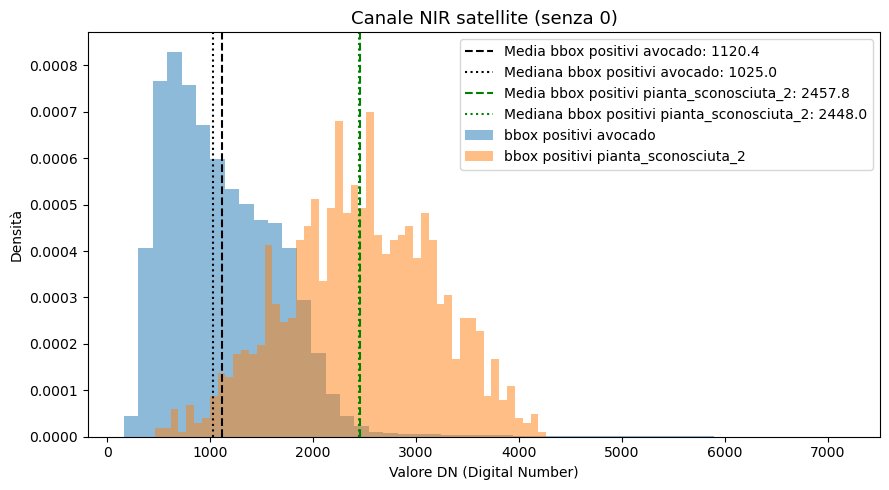
\includegraphics[width=0.9\textwidth]{capitoli/capitolo2/images/nir_pianta2_senza0.png}
    \end{minipage}
    \hfil 
    \begin{minipage}{0.45\textwidth}
    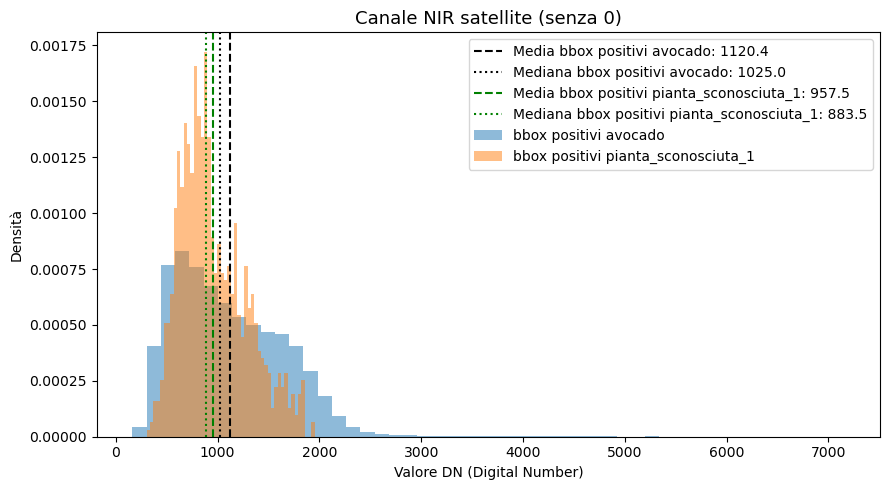
\includegraphics[width=0.9\textwidth]{capitoli/capitolo2/images/nir_pianta1_senza0.png}
    \end{minipage}
    \caption{Si mostrano i grafici NIR delle bbox delle tipologie di piante 1 e 2}
    \label{fig:grafici NIR pianta12}
\end{figure}
\begin{figure}[htbp]
    \centering
    \begin{minipage}{0.45\textwidth}
    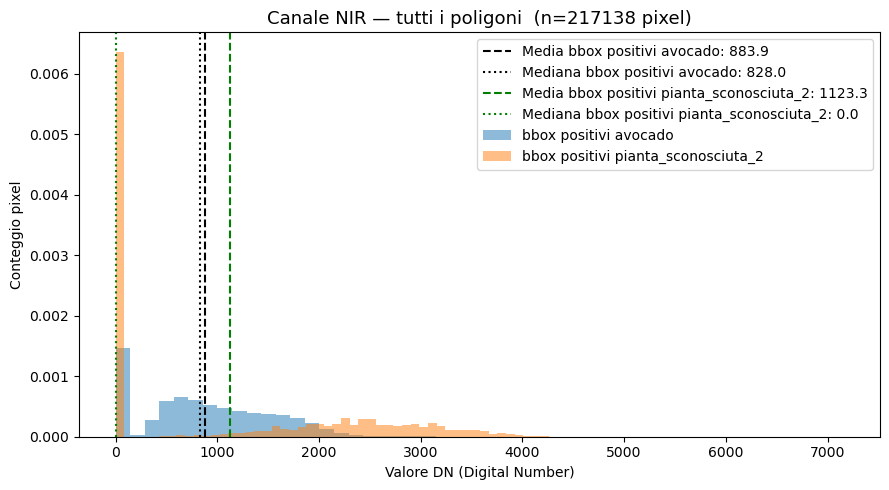
\includegraphics[width=0.9\textwidth]{capitoli/capitolo2/images/nir_pianta2.png}
    \end{minipage}
    \hfil 
    \begin{minipage}{0.45\textwidth}
    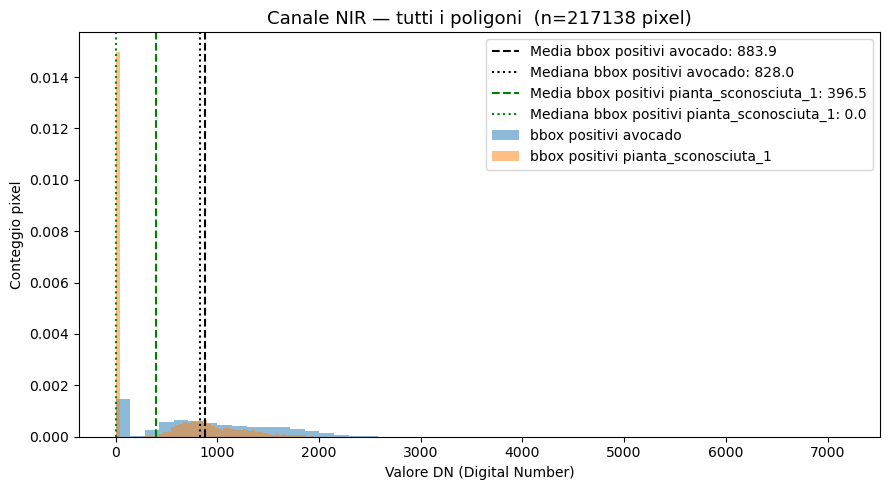
\includegraphics[width=0.9\textwidth]{capitoli/capitolo2/images/nir_pianta1.png}
    \end{minipage}
    \caption{Si mostrano i grafici NIR delle bbox delle tipologie di piante 1 e 2 togliendo i valori vicino allo 0}
     \label{fig:grafici NIR pianta12 senza0}
\end{figure}

Di seguito si mostrano i grafici \ref{fig:grafici SWIR pianta12} \ref{fig:grafici SWIR pianta12 senza0} anche per il campo SWIR sempre per le stesse tipologie.

\begin{figure}[htbp]
    \centering
    \begin{minipage}{0.45\textwidth}
    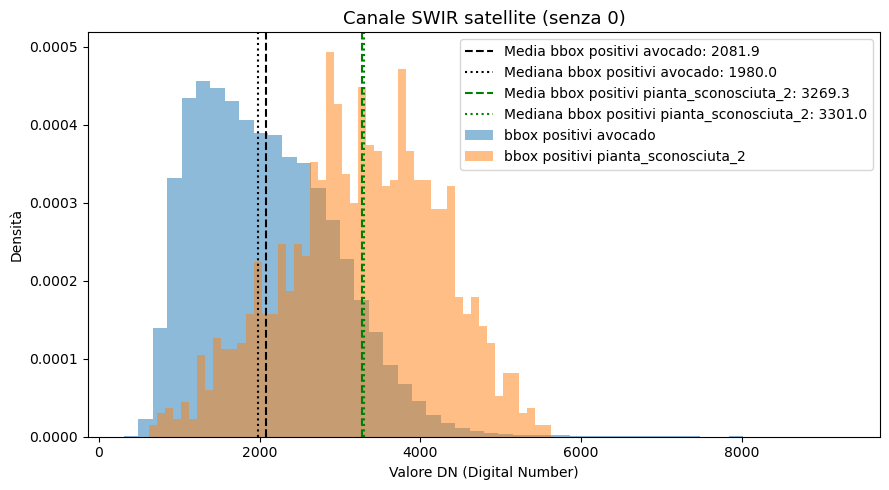
\includegraphics[width=0.9\textwidth]{capitoli/capitolo2/images/swir_pianta2_senza0.png}
    \end{minipage}
    \hfil 
    \begin{minipage}{0.45\textwidth}
    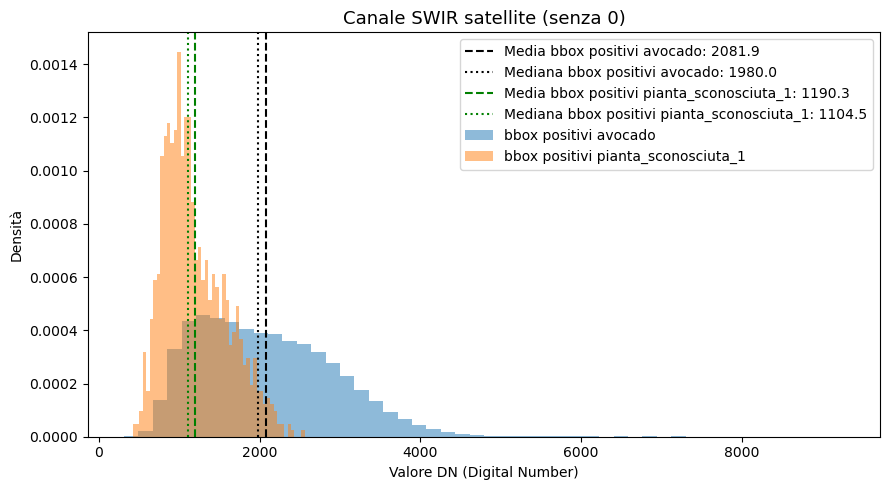
\includegraphics[width=0.9\textwidth]{capitoli/capitolo2/images/swir_pianta1_senza0.png}
    \end{minipage}
    \caption{Si mostrano i grafici SWIR delle bbox delle tipologie di piante 1 e 2}
    \label{fig:grafici SWIR pianta12 senza0}
\end{figure}
\begin{figure}[htbp]
    \centering
    \begin{minipage}{0.45\textwidth}
    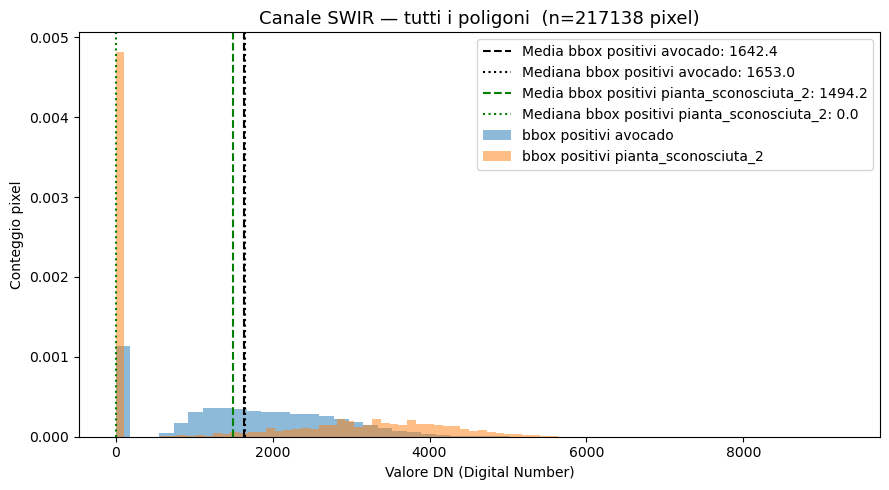
\includegraphics[width=0.9\textwidth]{capitoli/capitolo2/images/swir_pianta2.png}
    \end{minipage}
    \hfil 
    \begin{minipage}{0.45\textwidth}
    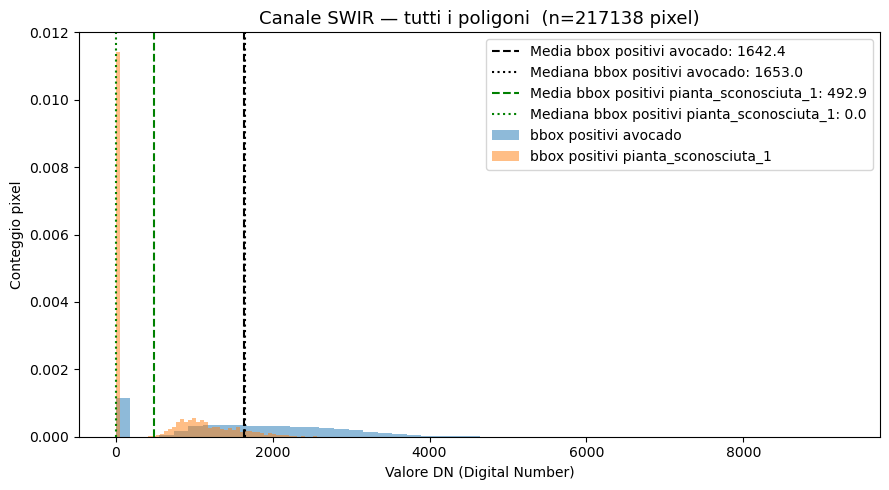
\includegraphics[width=0.9\textwidth]{capitoli/capitolo2/images/swir_pianta1.png}
    \end{minipage}
    \caption{Si mostrano i grafici SWIR delle bbox delle tipologie di piante 1 e 2 togliendo i valori vicino allo 0}
    \label{fig:grafici SWIR pianta12}
\end{figure}

Come si può osservare dai grafici \ref{fig:grafici SWIR pianta12} \ref{fig:grafici SWIR pianta12 senza0} \ref{fig:grafici NIR pianta12 senza0} \ref{fig:grafici NIR pianta12}  a tutte le tipologie 
di piante analizzate è possibile distinguere visivamente le distribuzioni.

Si afferma, inoltre, lo sbilanciamento del dataset per le classi. A tal riguardo si riporta una tabella che mostra che riporta il numero di Pixel per tipologia
\begin{table}[H]
\centering

\begin{tabular}{lc}
\hline
\textbf{Classe} & \textbf{Numero di Pixel} \\
\hline
Sfondo      & 113\,035 \\
Tipologia 1 & 135\,863 \\
Tipologia 2 & 1\,068 \\
Tipologia 3 & 6\,392 \\
Tipologia 4 & 40\,000 \\
\hline
\end{tabular}
\label{tab:support_classi}
\caption{Numero di campioni per ciascuna classe.}
\end{table}
Questo conferma che le proporzioni del dataset non sono distribuite
equamente tra il numero di pixel da confrontare tra le varie tipologie. Il che potrebbe portare a delle scarse performance del modello.


\section{Valutazione degli approcci possibili}

Per i compiti di classificazione nelle tipologie di piante si è scelto di adottare una Foresta Casuale \ref{subsec:foresta_casuale}.  
Rispetto all'utilizzo di una CNN (Convolutional Neural Network) per la classificazione di ogni pixel, la Foresta Casuale 
offre maggiore interpretabilità dei dati, richiede un numero di dati minore per l'allenamento e, infine, 
è computazionalmente più leggera. In questo caso l'utilizzo di una CNN sarebbe un aggravio delle performance e 
un aumento della complessità generale.


Successivamente si andrà ad applicare una Regressione Lineare 
\ref{subsec:regressione_lineare} per comprendere il numero di piante dato un 
agglomerato di pixel classificati pianta dalla Foresta Casuale. 

Poiché il dataset \cite{guillem_montalban_faet_2025_17866344} lavora solo con la banda infrarossa NIR si è scelto di addestrare 2 Foreste Casuali. 
Una lavorerà solo con la banda NIR e una lavorerà sia con la banda NIR che con la banda SWIR.

\section{Implementazione del modello}
\subsection{Foresta Casuale su immagini}
Si è andati a creare delle features derivate: media3x3, media7x7, std3x3 e std7x7 per ogni banda disponibile (quindi NIR e SWIR). Nello specifico si crea un immagine \texttt{.tiff} con 10 bande (media3x3rosso,media3x3verde,...).
Per costruire il dataset di addestramento, sono stati estratti i pixel all'interno delle bbox annotate per classe. I campioni così ottenuti vengono randomizzati per evitare correlazioni dovute all'ordine dei pixel.
Infine si allena la foresta.
Per entrambi i modelli è stato impostato un limite
di 70 alberi per Foresta (infatti indipendentemente dal superamento di questa soglia la bontà del modello non aumentava) e ed è stato impostato un vincolo 
in profondità per gli alberi decisionali di 23. Infatti non vi erano grossi differenze tra le profondità degli alberi della foresta e la loro performance.
Il dataset viene suddiviso in training set $(80\%)$, mentre
il restante è il test set $(20\%)$. La foresta casuale viene addestrata sul training, 
mentre i suoi risultati vengono testati sul test set per valutare la bontà del modello.




Per l'implementazione del codice è stato usato Python utilizzando la libreria Scikit-learn per la creazione della Foresta.


\subsection{Regressione lineare su dimensione pixel}

Al termine della classificazione si avrà un elenco di pixel che la macchina ha valutato come \texttt{pianta(di tipologia 1,2,3)} o \texttt{non pianta}.
Dato che una singola pianta è considerata come un agglomerato di pixel \texttt{pianta(della stessa tipologia)}, cioè un gruppo di pixel adiacenti, per risalire al numero di piante è necesssario lavorare sugli agglomerati stessi.\\
Un agglomerato è definito come un insieme massimale di pixel di classe \texttt{pianta} appartenenti a una singola tipologia, in cui ogni pixel è connesso ad almeno un altro pixel dell'insieme tramite adiacenza. \\
Per estrarre tutti gli agglomerati dall'immagine, si esegue una scansione completa dell'immagine.
Per contare i pixel presenti negli agglomerati si itera su tutti i pixel dell'immagine. Quando si trova un pixel \texttt{pianta} allora si esegue un BFS (Breadth First Search) dei pixel \texttt{pianta} vicini e si conta il numero dei pixel.
Si è pensato di effettuare attraverso il BFS anche la conta dei pixel del perimetro dell'agglomerato.
Per comprendere il numero di piante presenti in quell'insieme si è optato per l'impiego di una Regressione Lineare sugli agglomerati 
di pixel.
Il plot della regressione per la \texttt{tipologia avocado} è il seguente \ref{fig:grafico regressione}.
\begin{figure}[H]
    \centering
    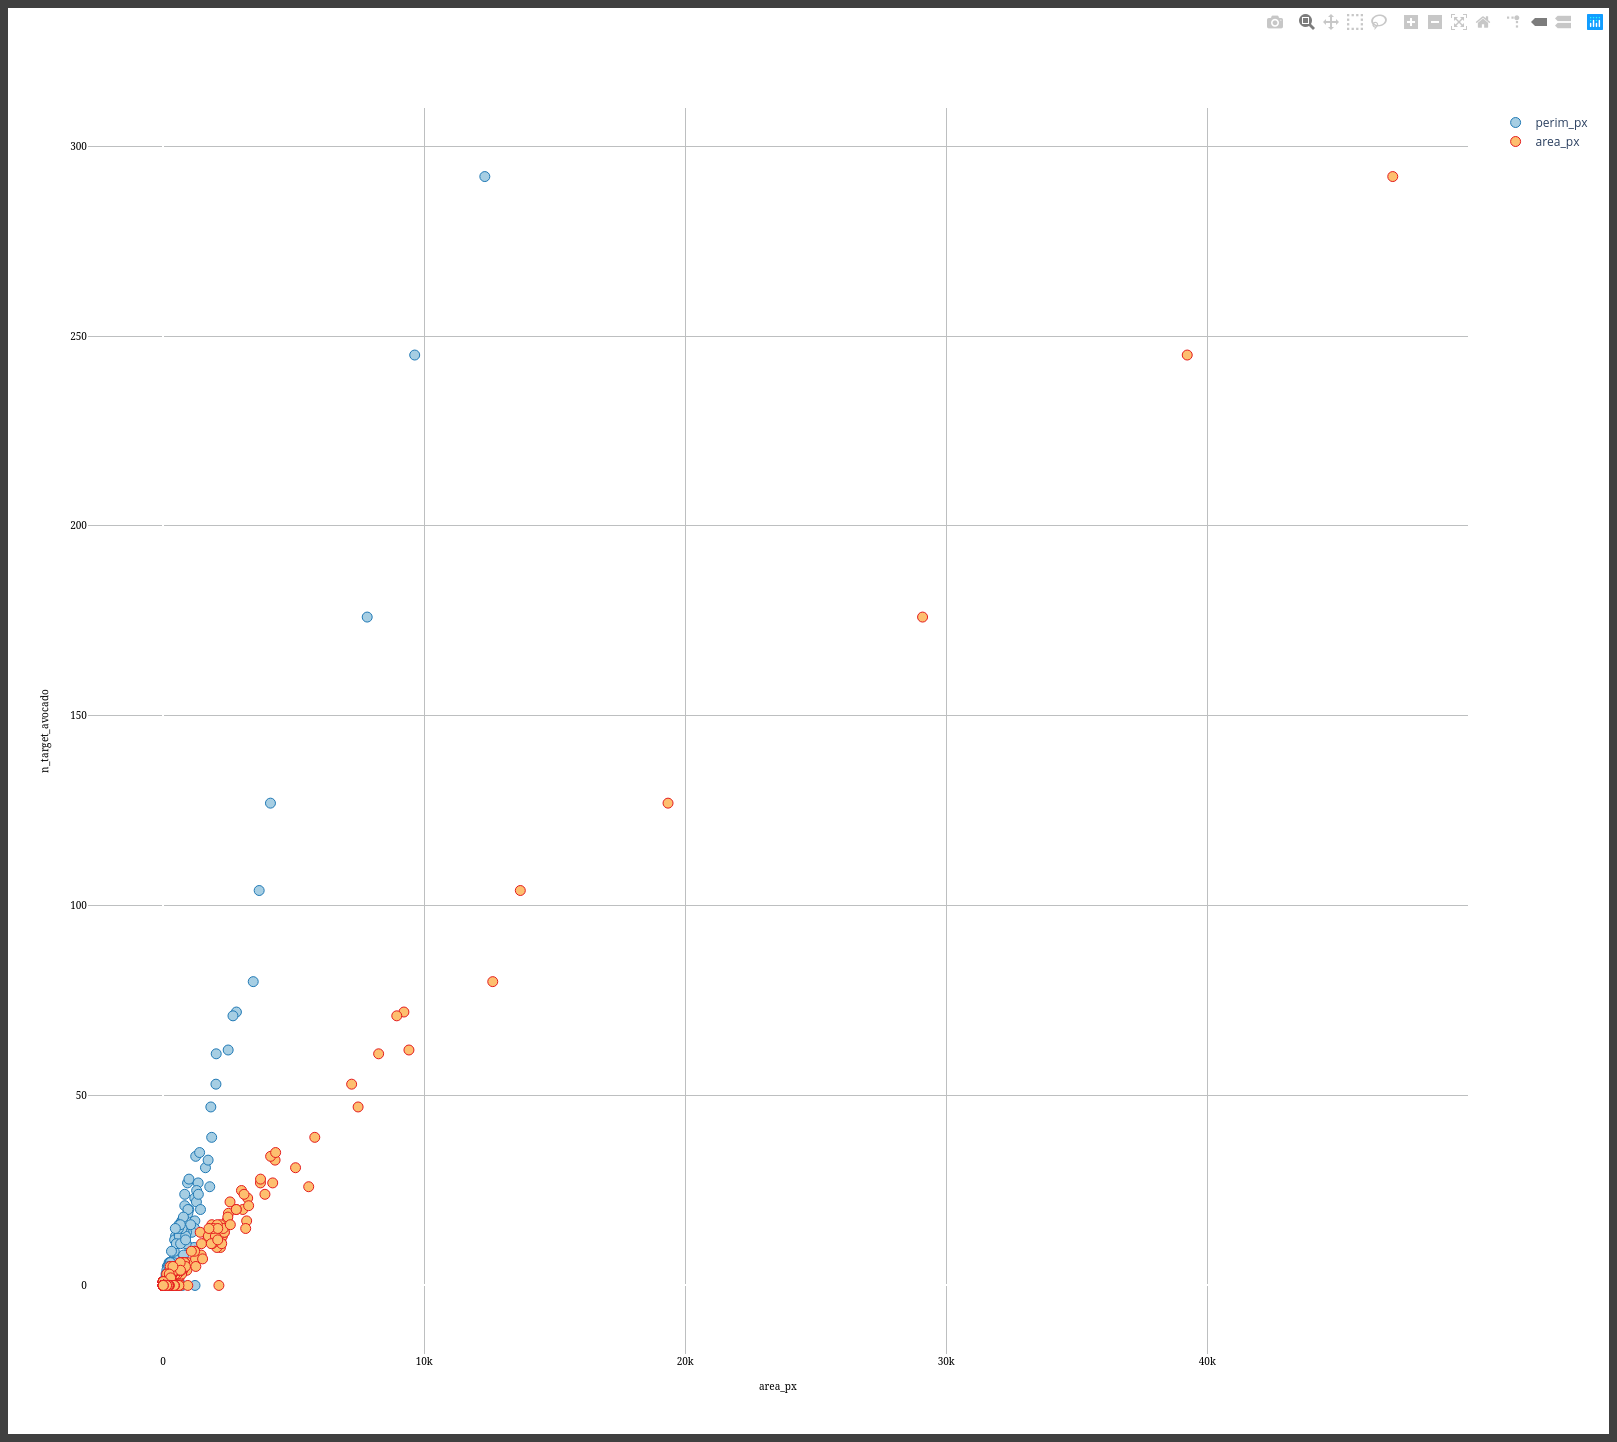
\includegraphics[width=0.5\textwidth]{capitoli/capitolo2/images/regressione.png}
    \caption{Visualizzazione del grafico con in arancione i punti che indicano il numero dei pixel di un agglomerato e in blu i punti del numero di pixel come perimetro dell'agglomerato}
    \label{fig:grafico regressione}
\end{figure}
Le formule delle rette di regressione trovate per l'area e il perimetro per la \texttt{tipologia avocado} sono rispettivamente:
\begin{align}
    y&=0.00636x-0.00812\\
    y&=0.0236x-0.239 
\end{align}
Si è deciso che il modello seguirà per la \texttt{tipologia avocado} solo la regressione dell'area dell'agglomerato poichè ha una 
accuratezza maggiore ($R^2=0.991$) rispetto al perimetro ($R^2=0.968$)\\

Si fa presente che la seguente regressione funziona solo se 1 pixel ha una singola pianta. 
Nel caso ci fossero delle piante annidate e che quindi 1 pixel contiene delle piante di varie tipologie la regressione 
andrebbe ad approssimare il numero di piante in modo grossolano ed errato.

\subsection{Modello NIR e SWIR}
Nel modello con NIR e SWIR si è andati ad usare entrambe la bande con un totale di 10 canali.
Questo è stato allenato con solo dataset di un immagine satellitare fornita dall'azienda con risoluzione $30cm/px$.
\subsection{Modello solo NIR}
Nel modello con solo NIR si è andati ad usare solo la banda NIR con un totale di 5 bande.
Questo modello è stato addestrato utilizzando lo stesso dataset del modello NIR e SWIR, però usando solo il canale NIR e il dataset \cite{guillem_montalban_faet_2025_17866344}.
La risoluzione satellitare del dataset fornito dall'azienda è di $30cm/px$. 
Non tutti i dataset sono normalizzati quindi si è proceduto con una normalizzazione della risoluzione.
È noto inoltre che nel dataset \cite{guillem_montalban_faet_2025_17866344} è stato usato il drone DJI Mavic 3 Multispectral. Ha volato con quota 14 m di altezza. 
La formula per trovare la risoluzione dei pixel è:
\[
GSD=\frac{H \cdot S_w}{f \cdot I_w}
\]
Dove $H$ è l'altezza in volo, $S_w$ è la larghezza del sensore, $f$ è la focale e $I_w$ è la larghezza immagine in pixel. Quindi la formula diventa:
\[
GSD=\frac{14000mm \cdot 17.3mm}{ 12mm \cdot 5280 px}=0.38 cm/px
\]
Di conseguenza:
\[ 
\text{FattorediScala}=\frac{GSD\text{ satellite}}{GSD\text{ drone}}=\frac{30cm/px}{0.38cm/px}=78.95
\]

In questo modo si è potuto comprendere quanto ridimensionare le immagini del dataset \cite{guillem_montalban_faet_2025_17866344} 
in modo da uniformarle al dataset satellitare fornito dall'azienda.

Questo modello, se ne deriva che, troverà una tipologia di pianta in più ovvero gli aranci presenti solo nel dataset \cite{guillem_montalban_faet_2025_17866344}.